\documentclass[aspectratio=169]{beamer}
\mode<presentation>
%\usetheme{Warsaw}
%\usetheme{Goettingen}
\usetheme{Hannover}
%\useoutertheme{default}

%\useoutertheme{infolines}
\useoutertheme{sidebar}
\usecolortheme{dolphin}

\setbeamersize{sidebar width left=0pt} % to remove the sidebar
\beamertemplatenavigationsymbolsempty % To remove the navigation symbols on the bottom right.
\setbeamersize{text margin left=10mm,text margin right=10mm} % Specify margins

\usepackage{amsmath}
\usepackage{amssymb}
\usepackage{enumerate}



%some bold math symbosl
\newcommand{\Cov}{\mathrm{Cov}}
\newcommand{\Var}{\mathrm{Var}}
\newcommand{\brho}{\boldsymbol{\rho}}
\newcommand{\bSigma}{\boldsymbol{\Sigma}}
\newcommand{\btheta}{\boldsymbol{\theta}}
\newcommand{\bbeta}{\boldsymbol{\beta}}
\newcommand{\bmu}{\boldsymbol{\mu}}
\newcommand{\bW}{\mathbf{W}}
\newcommand{\one}{\mathbf{1}}
\newcommand{\bH}{\mathbf{H}}
\newcommand{\by}{\mathbf{y}}
\newcommand{\bolde}{\mathbf{e}}
\newcommand{\bx}{\mathbf{x}}

\newcommand{\cpp}[1]{\texttt{#1}}

%--------------------------------------------------
\providecommand{\abs}[1]{\lvert#1\rvert}
\providecommand{\norm}[1]{\lVert#1\rVert}
\providecommand{\Blue}[1]{\textcolor{blue}{#1}}
\providecommand{\Red}[1]{\textcolor{red}{#1}}
\newcommand{\celsius}{\ensuremath{^\circ}C}
%------------------------------------------------------------------

\title{Lecture 17. Predicate Logic and Quantifiers (\S 1.5)}
%\author{ \includegraphics[width=.4\textwidth,height=.7\textheight]{lecture4-fig0.png} }
\date{ }

\begin{document}
\frame[plain]{\titlepage}

\begin{frame}[plain]{Predicates}
  
  \begin{itemize}
   \item  In previous lectures, we mentioned how sentences that involve a variable, such as $x$, need not be 
     statements.
     \begin{itemize}
      \item  For example, the sentence 
         ``{\bf The number $x+2$ is an even integer}'' is not necessary true or false
          unless we know what value is substituted for $x$.
      \item If we restrict our choices to integers, then when $x$ is replaced by
         $-7$, $1$, or $5$, for instance, the resulting statement is false. 
      \item When an even integer is substituted for $x$, however, the resulting proposition
         is true.
     \end{itemize}
     \pause 
    \item We can denote the sentence ``The number $x+2$ is an even integer'' by $P(x)$, 
    which is called a \Blue{propositional function} at $x$.
    \pause 
    \item {\bf Definition} A \Blue{predicate logic}~\footnote{Also, called as
    a \Blue{first-order logic}.} 
     is a declarative sentence whose truth value
       depends on one or more variables
    that becomes a statement
        when the variables in it  are replaced by 
           certain allowable choices.
           We will say {\bf predicate logic} as just {\bf predicate}.
           
     \item In the example above, $P(3)$ is false and $P(2)$ is true.
      
     \end{itemize}
 
     
\end{frame}

%\begin{frame}[plain]{}

%    A {\bf predicate logic} consists of two parts:
%       \begin{itemize}
%         \item {\bf Subject}: Subject is the main part of the statement.
%         \item {\bf Predicate}: A predicate can be defined as a relation, 
%         which binds two atoms together in a statement.
%       \end{itemize}
       
%   For example, in $P(x) = $ ``The number $x+2$ is an even integer'', 
%   $x+2$ is the \Blue{subject} of the statement and "the number is an even number"
 %  is the
 %   \Blue{predicate} that refers to a property that
%the subject of the statement can have.

%\medskip

%{\bf Remark}. We will say {\bf predicate logic} as just {\bf predicate}.
       
%\end{frame}

\begin{frame}[plain]{}

  {\bf Example 17.1.} Predicate $Q(x, y) =$ ``$x$ is heavier than $y$''. Then
         the statement $Q$(feather, brick) is false.
  \medskip
  \pause 
  
  {\bf Example 17.2.} Equations are predicates: If $E(x)$ stands for the equation
      \[ x^2-x-6 = 0, \]
      then $E(3)$ is true and $E(4)$ is false.
      %\pause
      
   %   \begin{center}
   %      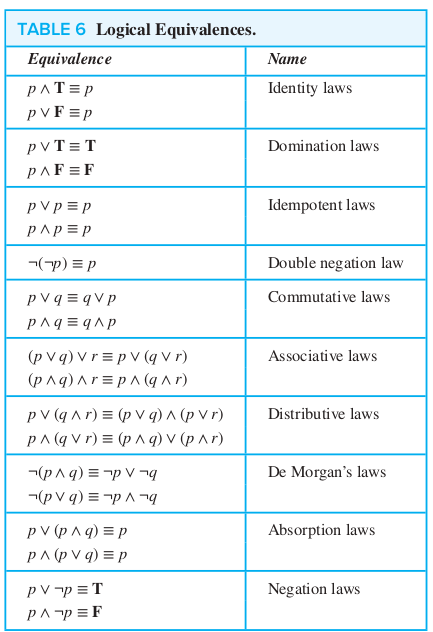
\includegraphics[height=2cm]{lecture15-fig1.png}
   %   \end{center}
      %https://ggc-discrete-math.github.io/logic.html#_predicates_and_quantifiers
  
  \vspace{1in}
  
      
\end{frame}


\begin{frame}[plain]{Quantifiers}
  
  We need \Blue{quantifiers} to express the meaning of English
        words including {\bf all} and {\bf some}: 
     \begin{itemize}
       \item ``\Red{All} men are Mortal.''
       \item  ``\Red{Some} cats do not have fur.''
     \end{itemize}
     \pause 
     
    The two most important quantifiers are: 
       \begin{itemize}
         \item \Blue{Universal Quantifier}, ``For All'', symbol: $\Blue{\forall}$
         \item \Blue{Existential Quantifier}, ``There Exists'', symbol: $\Blue{\exists}$
       \end{itemize}
      \pause 
      
      
     We write as in $\Blue{\forall x\in D,\, P(x)}$ and $\Blue{\exists x\in D,\, P(x)}$: \pause 
       \begin{itemize}[<+->]
         \item $\Blue{\forall x\in D,\, P(x)}$ = ``\Blue{For all $x$ in the domain $D$, $P(x)$ is true}''; i.e., 
              $P(x)$ is true for {\bf every} $x$ in 
             $D$.
         \item $\Blue{\exists x\in D,\, P(x)}$ = ``\Blue{There exists an $x$ in the domain $D$ 
            such that $P(x)$ is true}''; i.e.,  $P(x)$ is true for {\bf some} $x$ in $D$.
       \end{itemize}
\end{frame}

\begin{frame}[plain]{ }
  
  
  {\bf Universal Quantifier}: 
      $\Blue{\forall x\in D,\, P(x)}$ is read as ``\Blue{For \Red{all} $x$ in the domain $D$, $P(x)$ is true}'' 
      \medskip
      
   {\bf Example 17.3.}
     \begin{enumerate}[<+->]
      \item If $P(x)$ denotes ``$x>0$'' and its domain $D$ is the integers, then the statement
         [$\forall x\in D,\, P(x)$] is false.
      \item If $P(x)$ denotes ``$x>0$'' and $D$ is the positive integers, then the statement
         [$\forall x\in D,\, P(x)$] is true.
      \item If $P(x)$ denotes ``$x$ is even'' and $D$ is the integers, then the statement
         [$\forall x\in D,\, P(x)$] is false.
     \end{enumerate}
  
\end{frame}

\iffalse %%%%%%%%%
\begin{frame}[plain]{ }

 {\bf Example 17.4}. Let $P(x)$ be the statement $x+1>x$.
   Is this true for all integers $x$? A python code for this problem is
   \pause
   
    \begin{center}
      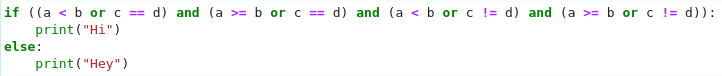
\includegraphics[height=5cm]{lecture15-fig2.png}
    \end{center}
% https://ggc-discrete-math.github.io/logic.html#_predicates_and_quantifiers

\end{frame}
\fi  %%%%%%%%%%

\begin{frame}[plain]{ }
  
     
   {\bf Existential Quantifier}: 
      $\Blue{\exists x\in D,\, P(x)}$ is read as ``\Blue{There \Red{exists} an $x$ in the domain $D$
      such that $P(x)$ is true}'' 
      \medskip
      
    {\bf Example 17.4.}
     \begin{enumerate}[<+->]
      \item If $P(x)$ denotes ``$x>0$'' and $D$ is the integers, then 
         [$\exists x\in D,\, P(x)$] is true. It is also true if $D$ is the positive integers.
      \item If $P(x)$ denotes ``$x<0$'' and $D$ is the positive integers, then 
         [$\exists x\in D,\, P(x)$] is false.
      \item If $P(x)$ denotes ``$x$ is even'' and $D$ is the integers, then 
         [$\exists x\in D,\, P(x)$] is true
     \end{enumerate}
\end{frame}


\iffalse%%%%%%%%%%%%%%%%%
\begin{frame}[plain]{}

  {\bf Example 17.6}. Let $P(x)$ be the statement $x^2=4$. 
  Is this true for at least one integer $x$? A python code for this problem is
  
  
  \begin{center}
      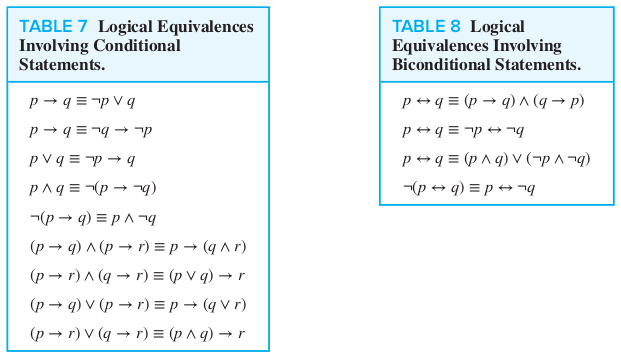
\includegraphics[height=5cm]{lecture15-fig3.png}
    \end{center}
% https://ggc-discrete-math.github.io/logic.html#_predicates_and_quantifiers
  
\end{frame}
\fi%%%%%%%%%%%%%%%%%%%%%%%%%

%\frame{ 
%  \frametitle{Thinking about Quantifiers}
  
%  \begin{itemize}[<+->]
%   \item When the domain of discourse is finite, we can think of
%  quantification as looping through the elements of the domain. 
%    \item To evaluate $\forall x\in D,\, P(x)$ loop through all $x$ in the domain $D$.
%     \begin{itemize}
%       \item If at every step $P(x)$ is true, then $\forall x\, P(x)$ is true.
%        \item If at a step $P(x)$ is false, then $\forall x\, P(x)$ is false and 
%        the loop terminates.
%     \end{itemize}
%   \item To evaluate $\exists x\, P(x)$ loop through all $x$ in the domain.
%       \begin{itemize}
%         \item If at some step, $P(x)$ is true, then $\exists x\, P(x)$ is true 
%           and the loop terminates.
%         \item  If the loop ends without finding an $x$ for which $P(x)$ is true, then
%              $\exists x\, P(x)$ is false.
%       \end{itemize}
%    \item Even if the domains are infinite, we can still think of the
%   quantifiers this fashion, but it would not be practical to
%   implement it this way.
%   \end{itemize}
%   }

\begin{frame}[plain]{ }
  
 
  The truth value of $\exists x\in D,\, P(x)$ and $\forall x\in D,\, P(x)$ depend on both
the propositional function (or predicate) $P(x)$ and on the domain $D$. \pause 
    \medskip
    
    {\bf Example 17.5.}
      \begin{enumerate}[<+->]
       \item If $D$ is the positive integers and $P(x)$ is the statement
	  ``$x < 2$'', then $\exists x\in D,\, P(x)$ is true, but $\forall x\in D,\, P(x)$ is false.
	\item  If $D$ is the negative integers and $P(x)$ is the statement
	    ``$x < 2$'', then both $\exists x\in D,\, P(x)$ and $\forall x\in D,\, P(x)$ 
	    are true.
	\item If $D$ consists of $3, 4,$ and $5$, and $P(x)$ is the statement
            ``$x> 2$'', then  both $\exists x\in D,\, P(x)$ and $\forall x\in D,\, P(x)$
             are true. But if
            $P(x)$ is the statement ``$x < 2$'', then both $\exists x\in D,\, P(x)$ and $\forall x\in D,\, P(x)$
            are false.
      \end{enumerate}


\end{frame}

\begin{frame}[plain]{}

{\bf Practice 17.6} Consider the predicate $R(x,y): 2x+y=0$, 
    where the domain of $x$ and $y$ is all rational numbers. 
    True or False?
 %   Write a python code for determining the truth values of the followings.
    \[ (a)\ R(0,0)\ \ \ (b)\ R(2, -1)\ \ \ (c)\ R(\frac{1}{5}, -\frac{2}{5})\ \ \ 
       (d)\ \exists y, R(0.2, y)\ \ \ (e)\ \forall y, R(7,y)
     \]

\vspace{1in}

 \end{frame}


\begin{frame}[plain]{Precedence of  Quantifiers}

The quantifiers \Blue{$\forall$} and \Blue{$\exists$} have higher precedence than
           all the logical operators.
  
  \begin{itemize}
    \item  For example, \Blue{$\forall x\, P(x)\vee Q(x)$} means \Blue{$(\forall x\, P(x))\vee Q(x)$}.
       \begin{itemize}
          \item Note: Here we omitted the domain $D$ assuming we already know what the domain is.
       \end{itemize}\pause 
    \item  \Blue{$\forall x\, (P(x)\vee Q(x))$} means something different. \pause 
  %  \item Unfortunately, often people wrongly write $\forall x\, P(x)\vee Q(x)$
  %	when they mean $\forall x\, (P(x)\vee Q(x))$.
    \item To avoid any confusion just put brackets right after
         every quantifier you use; i.e., \Blue{$\forall x\in D,\, \left[ P(x)\vee Q(x)\right]$} or
         \Blue{$\forall x \left[ P(x)\vee Q(x)\right]$}.
 \end{itemize}
\end{frame}



\begin{frame}[plain]{ }

 {\bf Example 17.7.} Translate the following sentence into
      predicate logic: 
        \begin{quote} 
         ``\emph{Every student in this class has taken
      a course in Java.}''\pause 
        \end{quote}
  
      \begin{itemize}
       \item {\bf Solution 1} If $D$ is all students in this class, define a
	predicate $J(x)$ denoting ``$x$ has taken a
	course in Java'' and translate as \Blue{$\forall x\in D,\, J(x)$}. \pause 
	\item {\bf Solution 2} But if $D$ is all people, also define a
	  predicate $S(x)$ denoting ``$x$ is a student in
         this class'' and translate as \Blue{$\forall x\in D,\, \left[ S(x)\rightarrow J(x)\right]$}.
  \end{itemize}
  
\vspace{.5in}

 
\end{frame}


\begin{frame}[plain]{Negating Quantified Expressions}
  
  \begin{itemize}
   \item Consider $\forall x\, J(x)$:\\
     ``\Blue{Every student in your class has taken a course in Java}.''\\
      Here \Red{$J(x)$} is ``\Blue{$x$ has taken a course in Java}'' and
      the domain is students in your class.
    \item  Negating the original statement gives \pause \\
     ``\Blue{It is not the case that every student in your class has taken Java}.''\\
    This implies that ``\Blue{There is a student in your class who
has not studied Java}.''
    \item Symbolically, 
    \Blue{$\neg\left[ (\forall x)\, J(x)\right]  \Leftrightarrow \pause (\exists x)\, (\neg J(x))$ }
 \end{itemize}
\end{frame}

\begin{frame}[plain]{}
  
  \begin{itemize}
   \item Now consider $\exists x\, J(x)$\\
     ``\Blue{There is a student in this class who has taken a course in Java}.''\\
      where \Red{$J(x)$} is ``\Blue{$x$ has taken a course in Java}'' and
      the domain is students in this class.
    \item  Negating the original statement gives  \pause \\
     ``\Blue{It is not the case that there is a student in this class who has taken Java}.''\\
    This implies that ``\Blue{Every student in this class has not studied Java}.''
    \item Symbolically, \Blue{$\neg\left[ (\exists x)\, J(x)\right] \Leftrightarrow \pause 
      (\forall x)\, (\neg J(x))$} 
 \end{itemize}
\end{frame}

\begin{frame}[plain]{Negation Rules  for Quantifiers}
   \Blue{
   \begin{eqnarray*}
     \neg\left[ (\forall x)\, P(x)\right] &\Leftrightarrow & (\exists x) (\neg P(x))\ \ \ \mbox{(universal negation)} \\
     \neg\left[ (\exists x)\, P(x) \right] &\Leftrightarrow & (\forall x) (\neg P(x)) \ \ \ \mbox{(existential negation)}
   \end{eqnarray*}
   }
   
   \medskip
   
 {\bf Example 17.8.} Express the statement in predicate logic and find its negation.
      \begin{center}
         ``\Blue{There does not exist anyone who likes skiing over magma.}''   
      \end{center}
     %MIT 2010 note ``Mathematics for Computer Science'', p19, Eq. (1.5)
 \medskip
 \pause
 
{\bf Practice 17.9} 
  Show that $\neg\left(\forall x [P(x)\rightarrow Q(x)]\right)$ and
    $\exists x [P(x)\wedge \neg Q(x)]$ are logically equivalent. %Rosen, 7ed, p48, Ex 22
 %  \item Let $Q(x,y)$ be the statement $x-y=4$. Write a python code of finding 
 %    the truth values of $Q(-1, 5), Q(4, 3),$ and $Q(-3, -7)$. 
 
\end{frame}

 \begin{frame}[plain]{}
 
 {\bf Practice 17.10}. 
  Let the domain be all faces of the following truncated {\bf icosahedron}.~\footnote{ 
    A solid figure having 20 faces. }
  \begin{columns}[c]
   \column{.4\textwidth}
      \begin{center}
     \includegraphics[height=2.7cm]{../../Lecture_F16/lecture6_fig1.png}
  \end{center}
   \column{.6\textwidth} 
    Consider the following predicates:
  {\small
  \begin{itemize}
   \item $P(x)$ = ``$x$ is a pentagon''
   \item $H(x)$ = ``$x$ is a hexagon''
   \item $B(x, y)$ = ``$x$ borders $y$''
  \end{itemize}
  }
  \end{columns}
  Here we say that two polygons \Blue{border each other} if they share an edge.
    Confirm that the following observations are true for any truncated icosahedron.
   \begin{itemize}
    \item No two pentagons border each other.
    \item Every pentagon borders some hexagon.
    \item Every hexagon borders another hexagon.
   \end{itemize}
   Write these statements in predicate logic, and negate them. 
   Simplify the negated statements so that no quantifier or connective lies within
   the scope of a negation. Translate your negated statement back into English.  
  
 \end{frame}


\end{document}
%%%%%%%%%%%%%%%%%%%%%%%%%

